\documentclass[11pt, xcolor={dvipsnames}, hyperref={colorlinks, allcolors=Blue}]{beamer}


% Packages
\usepackage{graphicx}
\usepackage{caption, subcaption}
\usepackage{tikz}
\usepackage{amsmath, amsfonts, amssymb}
\usepackage{bm}
\usepackage{booktabs}
\usepackage{apacite}
\usepackage{multirow}
\usepackage{multicol}
\usepackage{doi}
\usepackage{textpos}
\usepackage{lipsum}
\usepackage{amsfonts, amsmath}
\usepackage{wrapfig}
\usepackage{animate}
\usepackage{cleveref}


\renewcommand\doiprefix{}


\usepackage{tikz}
\usetikzlibrary{shapes, fit}





%%%%%%%%%%%%%%%%%%%%%%%%%%%%%%%%%%%%%%%%%%%%%%
% Custom commands
\newcommand\bc[1]{{\usebeamercolor[fg]{frametitle} {\textbf{#1}}}} % bold and color
\newcommand{\into}{\rightarrow}



%%%%%%%%%%%%%%%%%%%%%%%%%%%%%%%%%%%%%%%%%%%%%%
% Set Theme
\usetheme{Boadilla}
\usecolortheme{rose}

%%%%%%%%%%%%%%%%%%%%%%%%%%%%%%%%%%%%%%%%%%%%%%
% Make citation font tiny
\renewcommand{\bibliographytypesize}{\tiny}

%%%%%%%%%%%%%%%%%%%%%%%%%%%%%%%%%%%%%%%%%%%%%%
% Fonts
\usefonttheme{serif} % Serif font
\setbeamertemplate{enumerate items}[default] % Don't use bullets in enumerate.

%%%%%%%%%%%%%%%%%%%%%%%%%%%%%%%%%%%%%%%%%%%%%%%
% Remove navigation bar
\setbeamertemplate{navigation symbols}{}
%%%%%%%%%%%%%%%%%%%%%%%%%%%%%%%%%%%%%%%%%%%%%%


% Frontmatter
\title[ECON 8000 -  Lecture 11]{Lecture 11: Dynamic Programming II}
\author[University of Queensland]{Robert Garrard}
\date[\today]{} 


%%%%%%%%%%%%%%%%%%%%%%%%%%%%%%%

% Common commands

% Sets
\newcommand{\R}{\mathbb{R}}
\newcommand{\N}{\mathbb{N}}
\newcommand{\Z}{\mathbb{Z}}
\newcommand{\Q}{\mathbb{Q}}
\renewcommand{\P}{\mathbb{P}}
\newcommand{\E}{\mathbb{E}}

% Symbols
\renewcommand{\epsilon}{\varepsilon}
\renewcommand{\implies}{\Rightarrow}
\newcommand{\halmos}{\hfill$\blacksquare$}

% Vector notation
\renewcommand{\a}{\mathbf{a}}
\renewcommand{\b}{\mathbf{b}}
\newcommand{\h}{\mathbf{h}}
\newcommand{\x}{\mathbf{x}}
\newcommand{\X}{\mathbf{X}}
\newcommand{\y}{\mathbf{y}}
\newcommand{\z}{\mathbf{z}}
\renewcommand{\v}{\mathbf{v}}
\newcommand{\bepsilon}{\mathbf{\varepsilon}}
\newcommand{\bbeta}{\mathbf{\beta}}

% Matrices
\newcommand{\eyetwo}{\begin{pmatrix} 1 & 0\\ 0 & 1 \\ \end{pmatrix}} % I_2 identity matrix
\newcommand{\eyethree}{\begin{pmatrix} 1 & 0 & 0\\ 0 & 1 & 0\\ 0 & 0 & 1 \end{pmatrix}} % I_3 identity matrix
\newcommand{\zerotwo}{\begin{pmatrix} 0 & 0\\ 0 & 0 \\ \end{pmatrix}} % 2x2 Zero matrix
\newcommand{\zerothree}{\begin{pmatrix} 0 & 0 & 0\\ 0 & 0 & 0\\ 0 & 0 & 0 \end{pmatrix}} % 3x3 Zero matrix


% Misc

\newcommand{\innerprod}[2]{\langle #1, #2 \rangle}


%%%%%%%%%%%%%%%%%%%%%%%%%%%%%%%%

% Tikz
\usetikzlibrary{arrows,shapes,trees, positioning}

%%%%%%%%%%%%%%%%%%%%%%%%%%%%%%

\newcounter{Lecture}
\addtocounter{Lecture}{11}

\newcounter{exercise}
\newenvironment{exercise}[1][]{\refstepcounter{exercise}\par\medskip
   \noindent {\bc{Exercise}~\bc{\theLecture.\theexercise} #1}}{\medskip}


\begin{document}

\begin{frame}
\titlepage

%\begin{picture}(0,0)
%\put(35,-50){\hbox{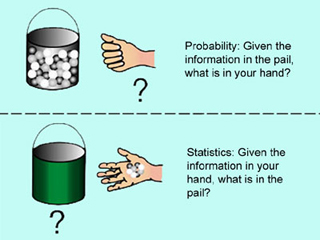
\includegraphics[width=0.8\textwidth, trim={0cm, 1cm, 0cm, 1cm}, clip]{prob_stats}}}
%\end{picture}

\end{frame}

%%%%%%%%%%%%%%%%%%%%%%%%%%%%%%%%
\begin{frame}{Previously}
Recall that some problem admit a recursive structure that we can describe with a \bc{Bellman equation}\medskip

\[V(k_{t}) = \underset{c_{t}}{\max} \ \left\{ U(c_{t}, k_{t}) + \beta V( g(c_{t}, k_{t})) \right\} \]
\bigskip

We saw that the Bellman operator was a contraction mapping with modulus $\beta$.\bigskip

We could solve the optimization problem numerically by performing \bc{value function iteration}.
\end{frame}

%%%%%%%%%%%%%%%%%%%%%%%%%%%%%%%%
\begin{frame}{Programming a Deterministic VFI}

Let's go through the process of programming a VFI in the context of a Ramsey growth model without labor. \bigskip

Recall that the problem is 

\begin{gather*}
V(k_{t}) = \underset{c_{t}}{\max} \quad \left\{U(c_{t}) + \beta V(k_{t+1})   \right\}\\
\text{s.t.} \quad c_{t} = Ak_{t}^{\alpha} + (1-\delta)k_{t} - k_{t+1}
\end{gather*}\bigskip

Let's parameterize the model to have: $U(c_{t}) = \log c_{t}$, $\beta=  0.95$, $\alpha = 1/3$, $\delta = 0.05$, $A = 1$.
\end{frame}

%%%%%%%%%%%%%%%%%%%%%%%%%%%%%%%%
\begin{frame}{Programming a Deterministic VFI}
\begin{figure}
	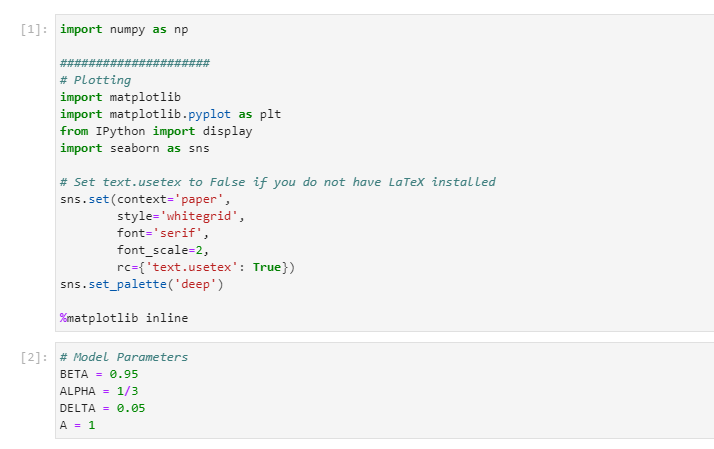
\includegraphics[width=0.95\textwidth]{Code1.png}
	\hfill
\end{figure}


\end{frame}

%%%%%%%%%%%%%%%%%%%%%%%%%%%%%%%%
\begin{frame}{Programming a Deterministic VFI}

Suppose we have have one state variable, $k_{t}$. Construct a grid of $n$ points for this variable: $[k_{0}, \dots, k_{n}]$. \bigskip

Recall that the steady state of this system is :

\[\bar{k} = \left [ \frac{\alpha\beta A}{1 - \beta(1-\delta)}  \right]^{\frac{1}{1-\alpha}} \qquad \bar{c} = A\bar{k}^{\alpha} - \delta \bar{k}\]
\bigskip

Let's center the grid around the steady state. Say, within 50\%, $k \in [(1-0.5)\bar{k}, (1+0.5)\bar{k}]$.

\begin{figure}
	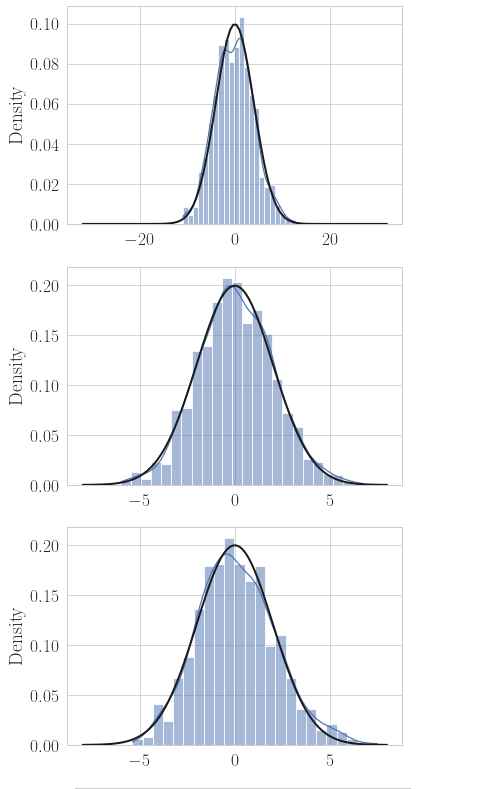
\includegraphics[width=0.95\textwidth]{Code2.png}
\end{figure}

\end{frame}

%%%%%%%%%%%%%%%%%%%%%%%%%%%%%%%%
\begin{frame}{Programming a Deterministic VFI}

Let $U$ be an $n\times n$ matrix for the period utility, where $U_{ij}$ is the payoff from having $i$ lots of the state variable today ($k_{t}$) and taking $j$ lots into tomorrow ($k_{t+1}$). \bigskip

We can find what the choice variable ($c_{t}$) must be today using the resource constraint.\bigskip

We also need to ensure that the constraints are satisfied. In particular, consumption must be non-negative. \bigskip

If $c_{t} > 0$, set $U_{ij} = \log(c_{t})$. If $c_{t} \leq 0$, set $U_{ij} = -\infty$.

\end{frame}

%%%%%%%%%%%%%%%%%%%%%%%%%%%%%%%%
\begin{frame}{Programming a Deterministic VFI}
\begin{figure}
	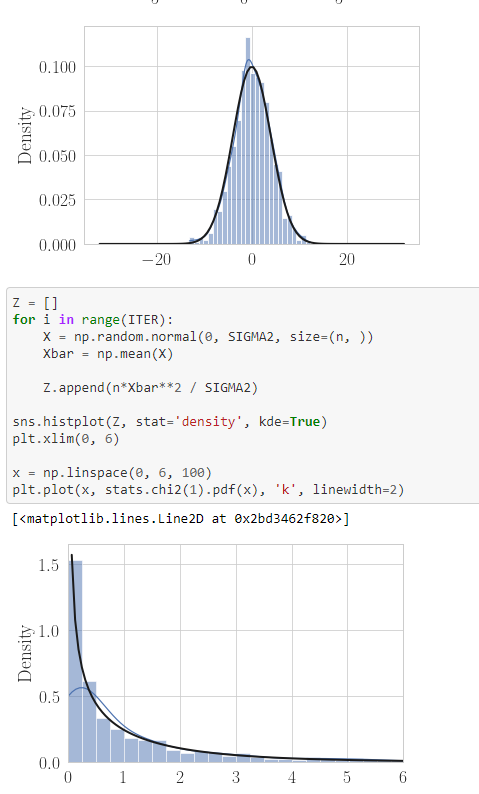
\includegraphics[width=0.95\textwidth]{Code3.png}
	\hfill
\end{figure}
\end{frame}

%%%%%%%%%%%%%%%%%%%%%%%%%%%%%%%%
\begin{frame}{Programming a Deterministic VFI}

Let our current guess for the value function be the $n\times 1$ vector $V = [V_1, \dots, V_n]^{\prime}$. Let $\mathbf{1}$ be an $n \times 1$ vector of ones. Then

\[
\begin{bmatrix}TV_{1} \\ \vdots \\ TV_{n} \end{bmatrix}
=
\underset{c_{t}}{\max} \left\{
	 \begin{pmatrix} U_{11} & \dots & U_{1 n}\\ \vdots & \dots & \vdots \\ U_{n1} & \dots & U_{nn} \end{pmatrix}  	
	+ \beta \begin{pmatrix} V_{1} & V_{2}& \dots & V_{n} \\ \vdots & \dots & \dots & \vdots \\ V_{1} & V_{2} & \dots & V_{n}  \end{pmatrix}  
	\right\}
 \]
\bigskip

Where the max operator is understood row-wise. We can write this more compactly as:

\[TV = \underset{c_{t}}{\max} \left\{U + \mathbf{1}V^{\prime} \right\}\]
\medskip

Begin with an initial guess, say $V^{0} = [0, \dots, 0]^{\prime}$, and iterate until convergence. 
\end{frame}

%%%%%%%%%%%%%%%%%%%%%%%%%%%%%%%%
\begin{frame}{Programming a Deterministic VFI}
\begin{figure}
	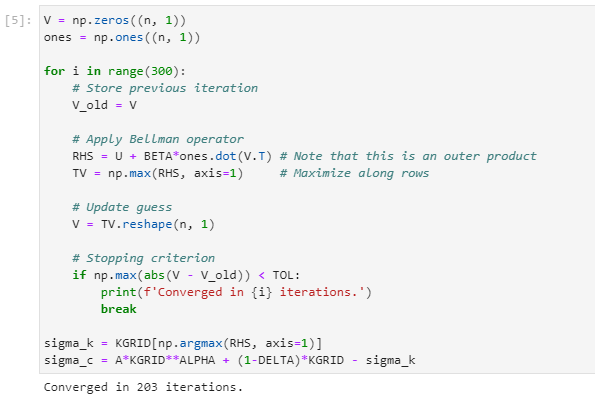
\includegraphics[width=0.95\textwidth]{Code4.png}
	\hfill
\end{figure}
\end{frame}

%%%%%%%%%%%%%%%%%%%%%%%%%%%%%%%%
\begin{frame}{Programming a Deterministic VFI}
\begin{figure}
	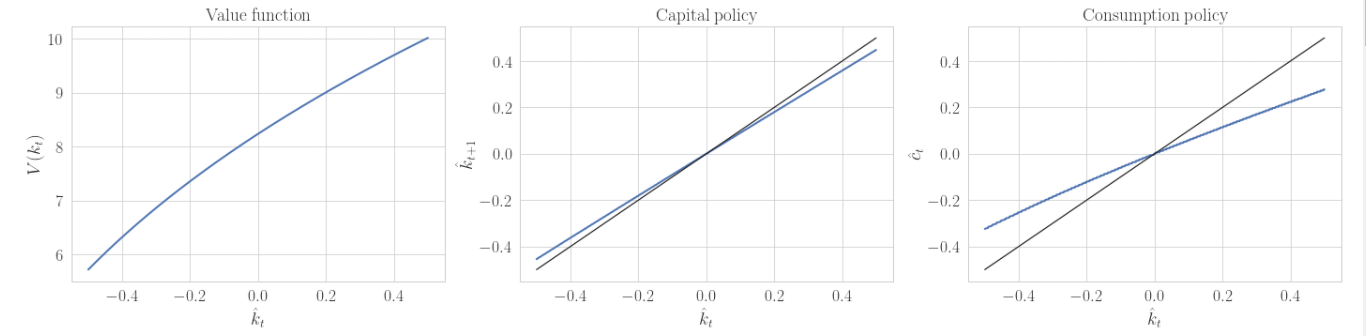
\includegraphics[width=0.95\textwidth]{Chart1.png}
	\hfill
\end{figure}

\end{frame}
%%%%%%%%%%%%%%%%%%%%%%%%%%%%%%%%
\begin{frame}{Programming a Stochastic VFI}
Recall the consumption/savings problem we explored with random income.

\begin{gather*}
V(k_{t}, y_{t}) = \max \quad \log(c_{t}) + \beta \mathbb{E}_{t} V(k_{t+1}, y_{t+1})\\
\text{s.t.} \quad c_{t} = (1+r)k_{t} + y_{t} - k_{t+1}\\
\mathbb{P}(y_{t} = 10) = 0.5 \quad \mathbb{P}(y_{t} = 0) = 0.5
\end{gather*}
\bigskip

We now have an extra state variable with two states, we'll call these states $\{1, 2\}$. In state 1 we get $y_t = 10$, in state 2 we get $y_t = 0$.\bigskip

Let's decompose this into having a different value function in each state, $V_{1}$ and $V_{2}$, and a different utility matrix 
in each state, $U_{1}$, $U_{2}$. \bigskip

Note that this model doesn't have a steady state, so we'll continue in levels rather than deviation from steady state.\bigskip

Let's use $r = 5\%$, and have our grid be $k_{t} \in [0, 300]$. 

\end{frame}

%%%%%%%%%%%%%%%%%%%%%%%%%%%%%%%%
\begin{frame}{Programming a Stochastic VFI}

\begin{figure}
	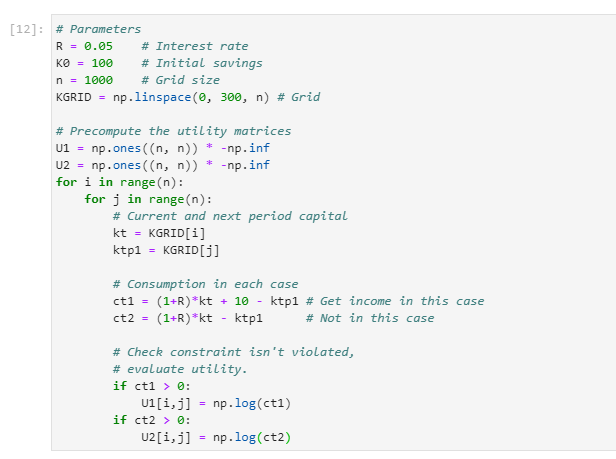
\includegraphics[height=0.8\paperheight]{Code5.png}
	\hfill
\end{figure}

\end{frame}

%%%%%%%%%%%%%%%%%%%%%%%%%%%%%%%%
\begin{frame}{Programming a Stochastic VFI}
Define the transition matrix to be the matrix of probabilities of transitioning from one state to another.

\[\mathcal{P} = \begin{pmatrix}\mathcal{P}_{11} & \mathcal{P}_{12}\\ \mathcal{P}_{21} & \mathcal{P}_{22} \end{pmatrix}\]
\bigskip

In our case, $\mathcal{P}_{11} = \mathcal{P}_{12} = \mathcal{P}_{21} = \mathcal{P}_{22} = \frac{1}{2}$. \bigskip

We split up the problem by conditioning on what state we're currently in. \bigskip

\[TV_{1} = \underset{c_{t}}{\max} \left \{  U_{1} + \beta \mathcal{P}_{11} \mathbf{1}V_{1}^{\prime} + \beta \mathcal{P}_{12} \mathbf{1}V_{2}^{\prime}  \right\} \]
\[TV_{2} = \underset{c_{t}}{\max} \left \{  U_{2} + \beta \mathcal{P}_{21} \mathbf{1}V_{1}^{\prime} + \beta \mathcal{P}_{22} \mathbf{1}V_{2}^{\prime}  \right\} \]

\end{frame}

%%%%%%%%%%%%%%%%%%%%%%%%%%%%%%%%
\begin{frame}{Programming a Stochastic VFI}
Stacking these together gives
\medskip

\[ 
\begin{bmatrix}TV_1 \\ TV_2 \end{bmatrix} = \underset{c_{t}}{\max} \ \left\{
\begin{bmatrix}U_1 \\ U_2 \end{bmatrix} + \beta (\mathcal{P} \otimes \mathbf{1})
\begin{bmatrix}V_{1}^{\prime} \\ V_{2}^{\prime}\end{bmatrix}
\right\}
\]
\bigskip

Again, max is row-wise. On the LHS, we have a $2n\times 1$ vector. We just need to split it in half to retrieve our value function.\bigskip

Iterate, and stop when the max across all entries in the LHS is within tolerance.
\end{frame}

%%%%%%%%%%%%%%%%%%%%%%%%%%%%%%%%
\begin{frame}{Programming a Stochastic VFI}

\begin{figure}
	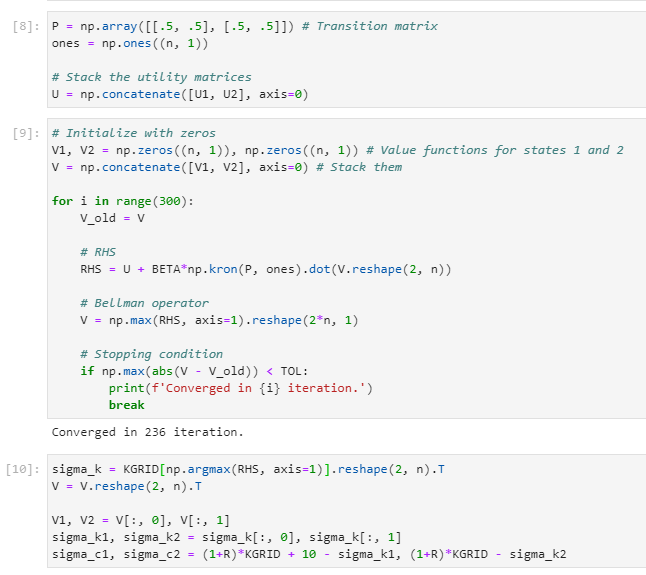
\includegraphics[height=0.8\paperheight]{Code6.png}
	\hfill
\end{figure}

\end{frame}

%%%%%%%%%%%%%%%%%%%%%%%%%%%%%%%%
\begin{frame}{Programming a Stochastic VFI}

\begin{figure}
	\centering
	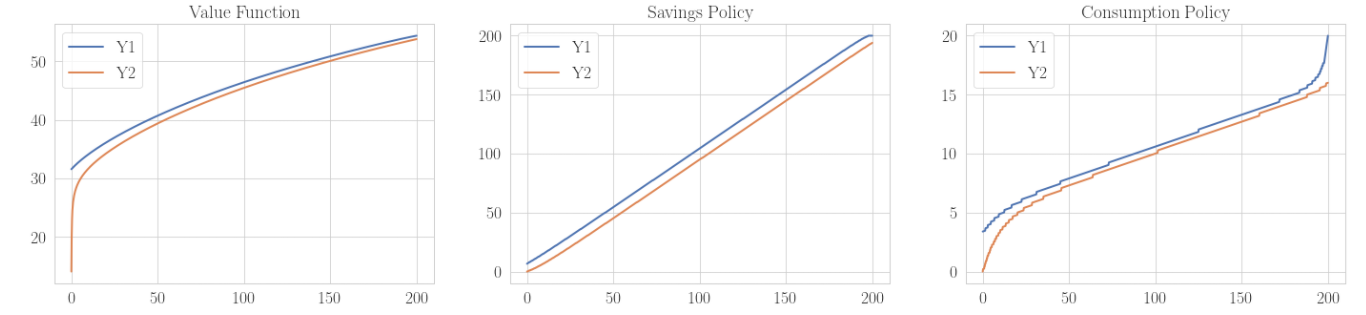
\includegraphics[width=\textwidth]{Chart2.png}
	\caption{Value and policy functions}
\end{figure}
\begin{figure}
	\centering
	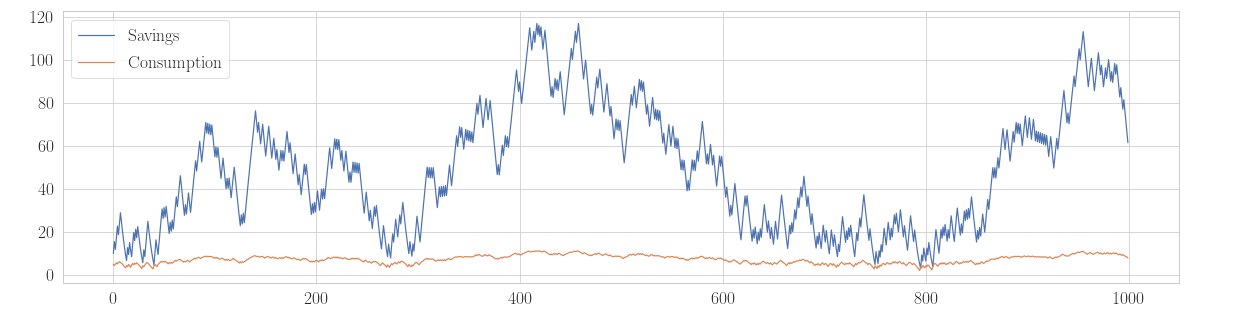
\includegraphics[width=\textwidth]{Chart3.png}
	\caption{Simulation for 1000 periods. $K_0 = 10$.}
\end{figure}

\end{frame}

%%%%%%%%%%%%%%%%%%%%%%%%%%%%%%%%
\begin{frame}{Static Variables}
What if we want to include extra variables that are chosen within each period? E.g.\bigskip

\begin{gather*}
\underset{\{c_{t}, \ell_{t}, k_{t+1}\}}{\max} \quad \sum_{t=0}^{\infty} \beta^{t} U(c_{t}, \ell_{t}) \\
\text{s.t.}\quad c_{t} + k_{t+1} = F(k_{t}, \ell_{t}) + (1-\delta)k_{t}
\end{gather*}
\end{frame}

%%%%%%%%%%%%%%%%%%%%%%%%%%%%%%%%
\begin{frame}{Static Variables}
Recall that that the first order condition for labor is:\medskip

\[\frac{U_{\ell}(c_{t}, k_{t})}{U_{c}(c_{t}, \ell_{t})} = F_{\ell}(k_{t}, \ell_{t})\]
\bigskip

Solve this first order condition for labor in terms of the control and state: $\ell_{t} = \ell(c_{t}, k_{t})$, and include it as a constraint in the problem\medskip

\[V(k_{t}) = \underset{c_{t}}{\max} \ \left\{  U(c_{t}, \ell(c_{t}, k_{t})) + \beta V\left( g(c_{t}, k_{t})\right)  \right\} \]\medskip

If you can't solve for $\ell(c_{t}, k_{t})$ analytically, use a numerical solver at each point of your grid.
\end{frame}

%%%%%%%%%%%%%%%%%%%%%%%%%%%%%%%%
\begin{frame}{Static Variables}
Let's solve the deterministic growth model with labor supply:

\begin{gather*}
V(k_{t}) = \underset{c_{t}}{\max} \ \left\{\log(c_{t}) + \eta \log (1-\ell_{t}) + \beta V(k_{t+1}) \right\}\\
\text{s.t.} \quad c_{t} = Ak_{t}^{\alpha}\ell_{t}^{1-\alpha} + (1-\delta)k_{t} - k_{t+1}
\end{gather*}
\bigskip

with $\eta = 2$, $\alpha=1/3$, $\beta = 0.95$, $\delta=0.05$.\bigskip

Note the steady state is:

\begin{align*}
&\bar{\ell} = \frac{1}{1 + \frac{\eta}{1-\alpha} ( 1 - \frac{\alpha \beta \delta}{1 - \beta(1 - \delta})}\\
&\bar{k} = \bar{\ell}\left[ \frac{\alpha\beta A}{1 - \beta(1-\delta)}\right]^{\frac{1}{1-\alpha}}\\
&\bar{c} = A\bar{k}^{\alpha}\bar{\ell}^{1-\alpha} - \delta \bar{k}
\end{align*}
\end{frame}

%%%%%%%%%%%%%%%%%%%%%%%%%%%%%%%%
\begin{frame}{Static Variables}

\begin{figure}
	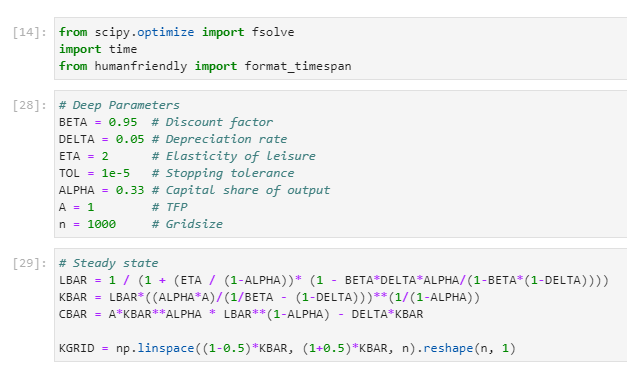
\includegraphics[width=0.9\textwidth]{Code7.png}
	\hfill
\end{figure}

\end{frame}

%%%%%%%%%%%%%%%%%%%%%%%%%%%%%%%%
\begin{frame}{Static Variables}

\begin{figure}
	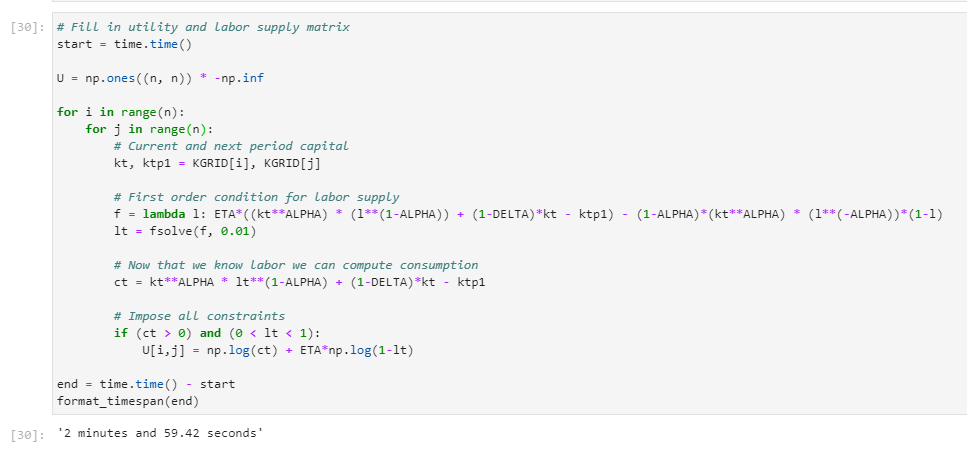
\includegraphics[width=\textwidth]{Code8.png}
	\hfill
\end{figure}

\end{frame}
%%%%%%%%%%%%%%%%%%%%%%%%%%%%%%%%
\begin{frame}{Static Variables}

\begin{figure}
	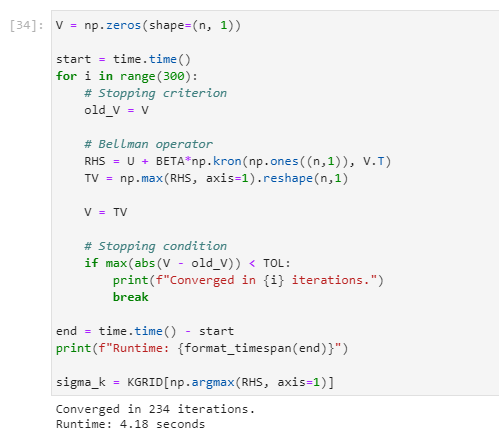
\includegraphics[height=0.8\paperheight]{Code9.png}
	\hfill
\end{figure}

\end{frame}
%%%%%%%%%%%%%%%%%%%%%%%%%%%%%%%%
\begin{frame}{Static Variables}

\begin{figure}
	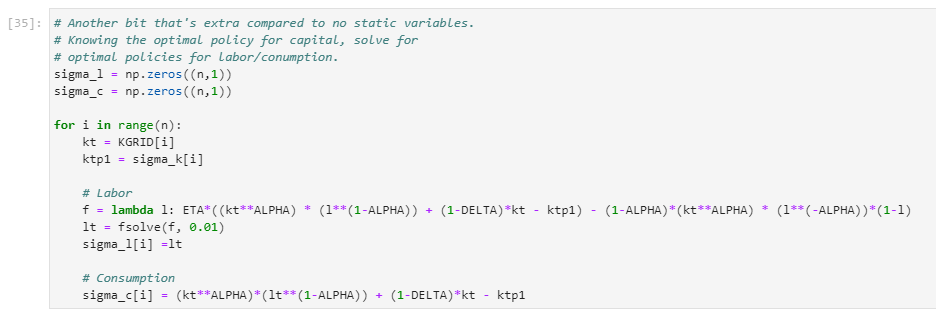
\includegraphics[width=\textwidth]{Code10.png}
	\hfill
\end{figure}
\end{frame}
%%%%%%%%%%%%%%%%%%%%%%%%%%%%%%%%
\begin{frame}{Static Variables}

\begin{figure}
	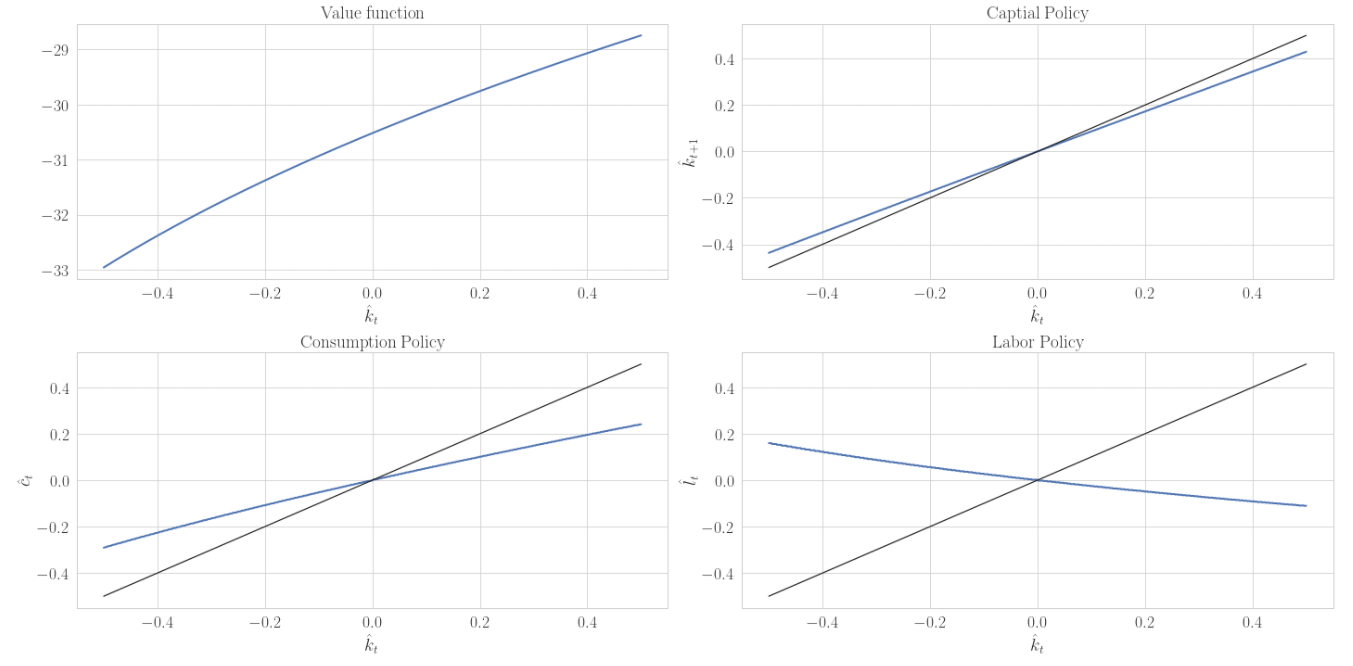
\includegraphics[width=\textwidth]{Chart4.png}
	\caption{Value and policy functions for growth model with labor}
\end{figure}
\end{frame}

%%%%%%%%%%%%%%%%%%%%%%%%%%%%%%%%
\begin{frame}{Discretizing an AR(1)}
When we model the process for TFP, it's convenient to specify an AR(1). For example, in a stochastic growth model:

\begin{gather*}
\underset{\{c_{t}, k_{t+1}\}}{\max} \quad \sum_{t=0}^{\infty} \beta^{t} \log(c_{t}) \\ 
\text{s.t.} \quad c_{t} + k_{t+1} = e^{z_{t}} k_{t}^{\alpha} + (1-\delta) k_{t}\\
z_{t+1} = \rho z_{t} + \epsilon\\
\epsilon \sim N(0, \sigma_{\epsilon}^{2})
\end{gather*}

To use our existing methods, we need to know the transition probabilities 

\[\P(z_{t+1} = x \ | \ z_{t} = y) \]

\end{frame}

%%%%%%%%%%%%%%%%%%%%%%%%%%%%%%%%
\begin{frame}{Discretizing an AR(1)}

We can use Tauchen's (1986, Econ. Lett.) method. \bigskip

Let our grid be $\lambda_{1} < \dots < \lambda_{m}$, evenly spaced around the mean of $z$ (0 in this case). Using the fact that $\epsilon$ is normal gives us an approximation:

\[
\mathcal{P}_{ij} \approx
\begin{cases}
\Phi( \frac{\lambda_{1} + w/2 - \rho \lambda_{i}}{\sigma_{\epsilon}} ) & \text{if } j = 1\\
\Phi( \frac{\lambda_{1} + w/2 - \rho \lambda_{i}}{\sigma_{\epsilon}} ) - \Phi( \frac{\lambda_{1} - w/2 - \rho \lambda_{i}}{\sigma_{\epsilon}} )& \text{if } 1 < j < m\\
1 - \Phi( \frac{\lambda_{1} - w/2 - \rho \lambda_{i}}{\sigma_{\epsilon}} ) & \text{if } j=m
\end{cases}
\]
\medskip

Where $w = \lambda_{i} - \lambda_{i-1}$ is the grid's mesh. 
\end{frame}

%%%%%%%%%%%%%%%%%%%%%%%%%%%%%%%%
\begin{frame}{Discretizing an AR(1)}
Now that we have productivity shocks, we can talk about what happens when we start in the steady state and are hit by a shock of a particular size (say 1 standard deviation). \bigskip

\begin{figure}
	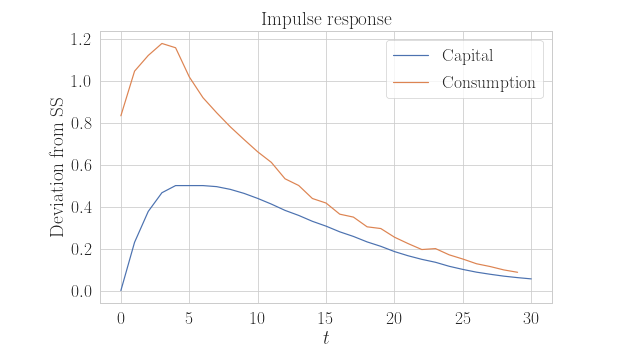
\includegraphics[width=0.75\textwidth]{Chart5.png}
\end{figure}
\end{frame}

%%%%%%%%%%%%%%%%%%%%%%%%%%%%%%%%
\begin{frame}{Learning Outcomes}

\bc{You should be able to:}

\begin{itemize}
	\item Numerically solve an optimization problem with value function iteration.
	\item Construct an appropriate transition matrix for random quantities.
\end{itemize}
\end{frame}

\end{document}	
